\documentclass[11pt]{article}
% \usepackage[french]{babel}
%  \usepackage{DejaVuSans}
%  \usepackage{libertine}
%  \renewcommand*\rmdefault{cmfib} 
% \usepackage[default]{cantarell}

% \usepackage[T1]{fontenc}
% \renewcommand{\rmdefault}{cmss}  
% \fontencoding{T1}
%   \fontfamily{cmss}
%   \fontseries{m}
%   \fontshape{n}
%   \fontsize{10}{15}
% \renewcommand*\familydefault{cmss}
%   \selectfont
% \usepackage[utf8]{inputenc} 
\usepackage{array, xcolor, lipsum, bibentry}
\usepackage[margin=2.4cm]{geometry} 
\usepackage{longtable}
\usepackage{fancyheadings}
 \pagestyle{fancyplain}
 \fancyhead{}
\fancyfoot{}
\renewcommand{\headrulewidth}{0pt}
\cfoot{\thepage}
\rfoot{\scriptsize \selectfont Iliya Enchev \longdate{\today}}
% \usepackage{helvet}
% \usepackage[french]{babel}
% \usepackage[T1]{fontenc}
% \usepackage[utf8]{inputenc}

% \usepackage[T1]{fontenc}
\usepackage{graphicx}
\usepackage[light,math]{iwona} 
% \usepackage{DejaVuSans}
%   \renewcommand{\rmdefault}{cmss}  
%   \renewcommand{\sfdefault}{cmr}
%   \renewcommand{\ttdefault}{ptm}

%     \usepackage{titlesec}
%     \titleformat{\section}{\large\bfseries}{\thesection}{1em}{}

\newcommand{\addphoto}[2]{%
  \smash{%
    \makebox[0pt][l]{%
      \raisebox{#1pt}{%
        \hspace{#2pt}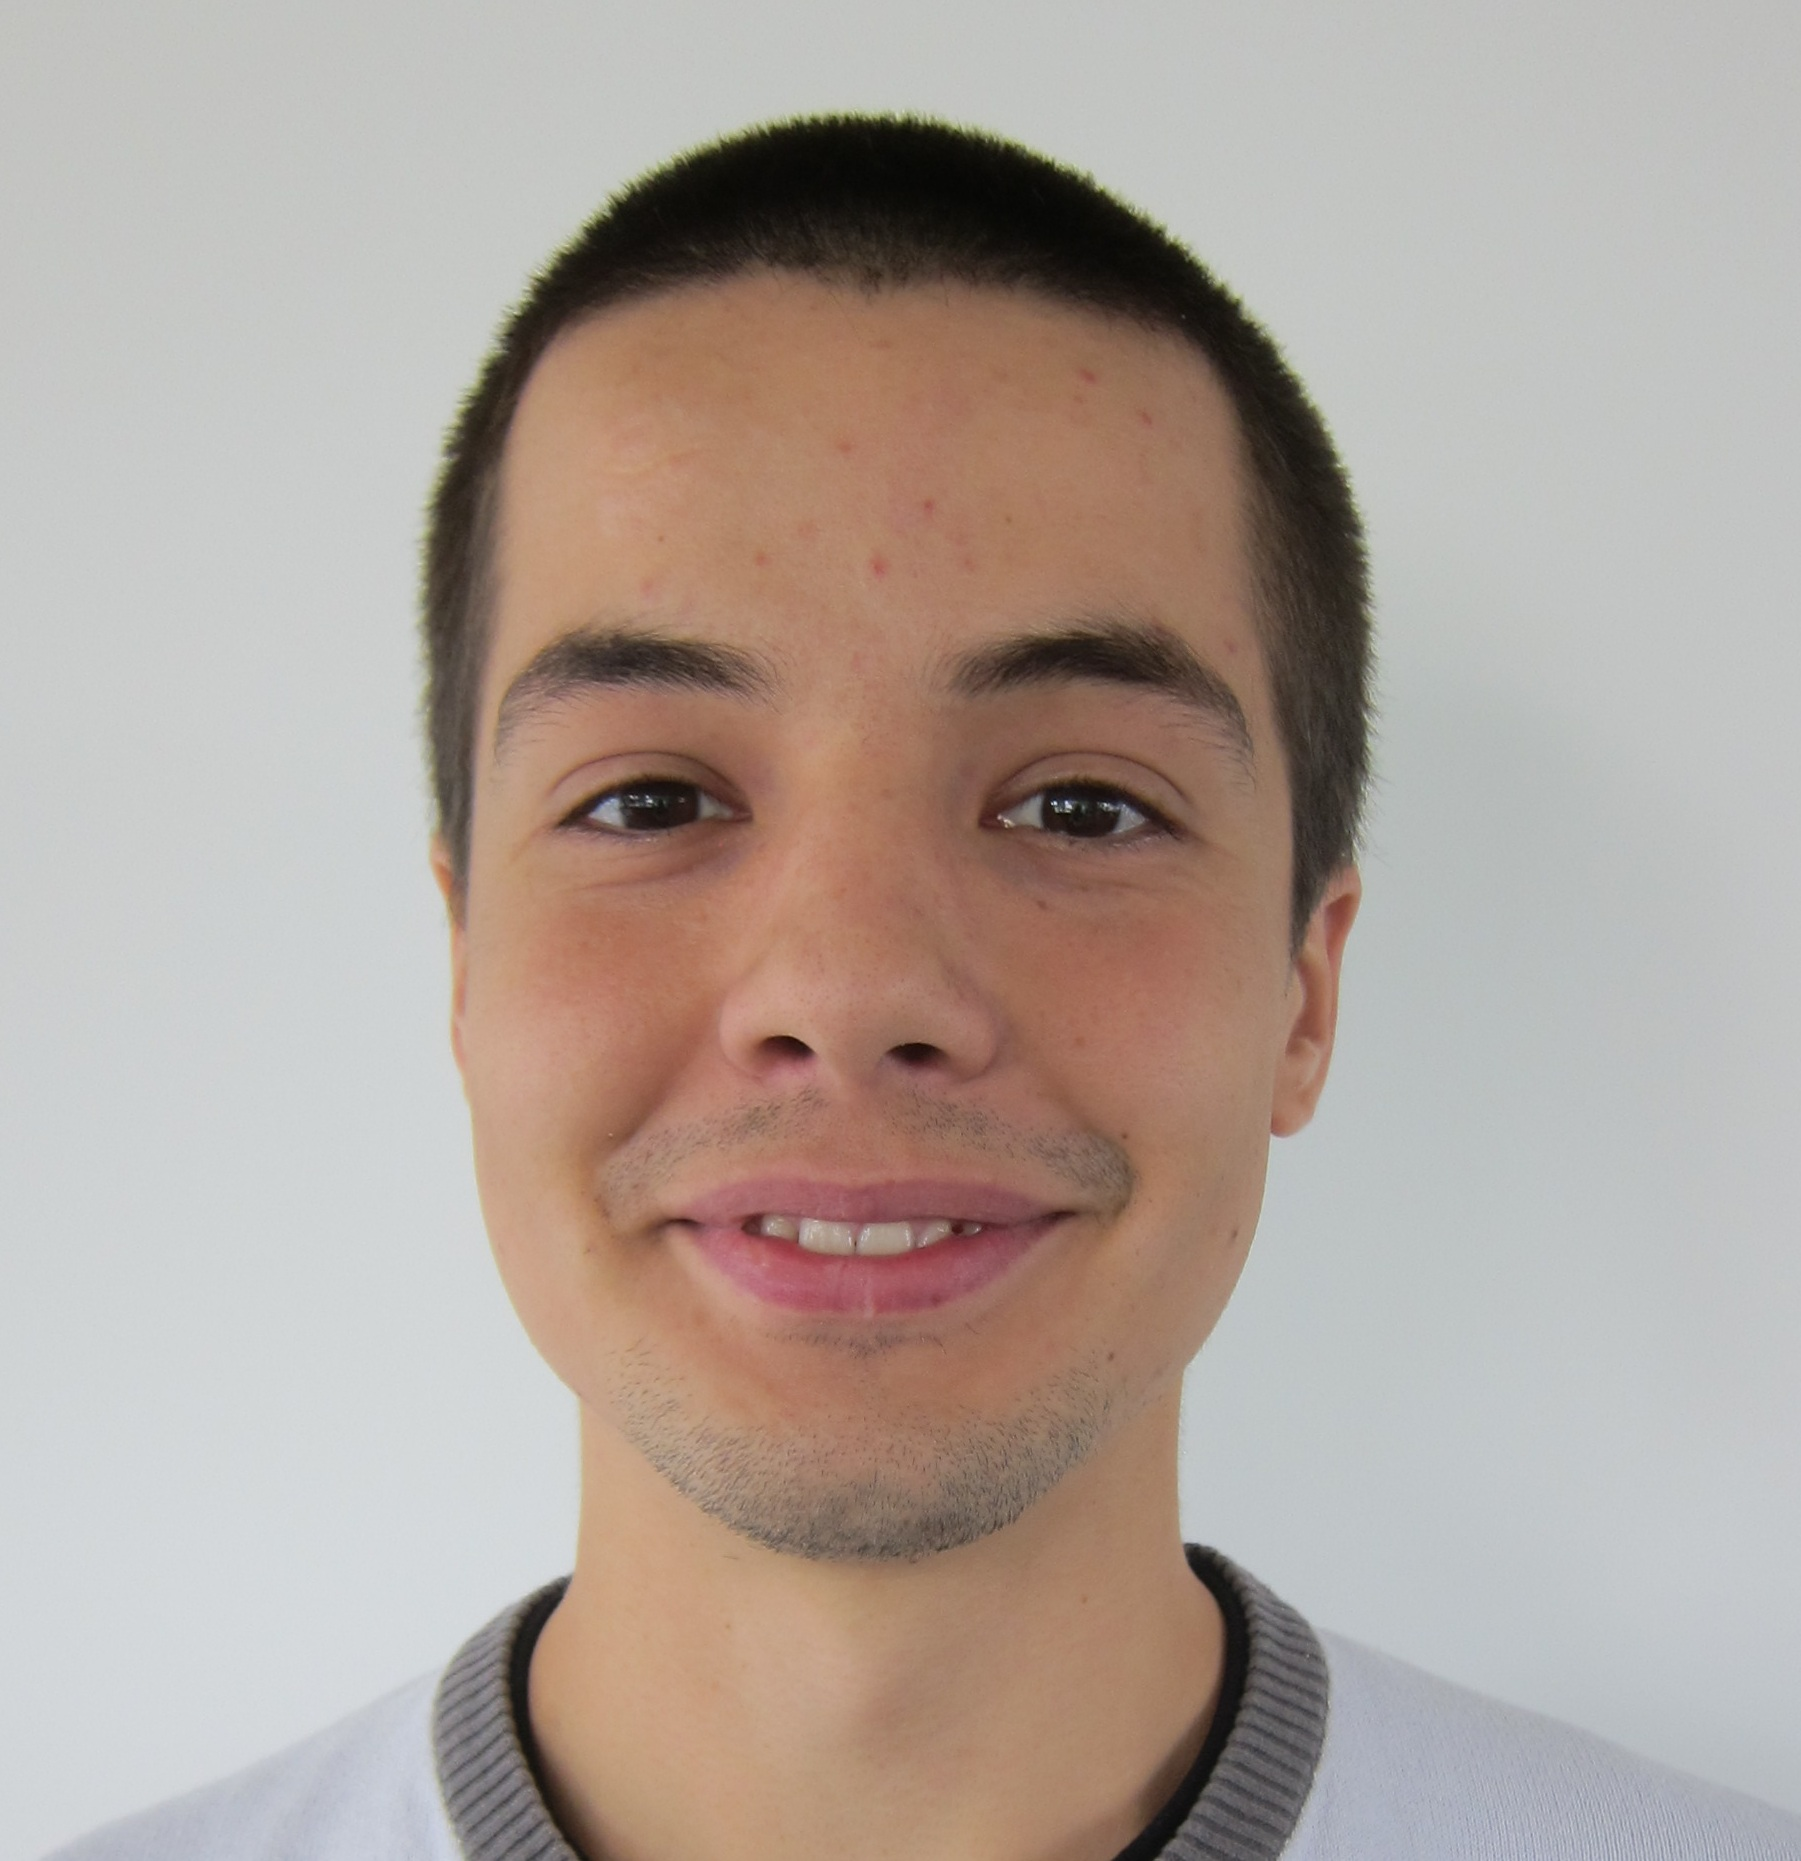
\includegraphics[width=3.7cm]{IMG_9061cropped3}%
      }%
     }%
  }%
}

%ptm phv pcr 
% \renewcommand{\rmdefault}{iwona}
% \renewcommand{\sfdefault}{iwona}
\usepackage[nodayofweek]{datetime}
\title{\bfseries\huge Iliya Stefanov Enchev\\
\addphoto{10}{138}}
\author{iliyastefanov@gmail.com}
\date{\today}
% \addphoto{5}{150}

\definecolor{lightgray}{gray}{0.8} 
\newcolumntype{L}{>{\raggedleft}p{0.17\textwidth}}
\newcolumntype{R}{p{0.8\textwidth}}
\newcommand\VRule{\color{lightgray}\vrule width 0.5pt}


% \begin{filecontents}{publication.bib}
% @article{lamport1986latex,
%   title={LaTEX: User's Guide \&amp; Reference Manual},
%   author={Lamport, L.},
%   year={1986},
%   publisher={Addison-Wesley}
% }
% @book{knuth2006art,
%   title={The art of computer programming: Generating all trees: history of combinatorial generation},
%   author={Knuth, D.E.},
%   volume={4},
%   year={2006},
%   publisher={addison-Wesley}
% }
% \end{filecontents} 

\begin{document}
% \addphoto{5}{150}


% 
\includegraphics{picture.jpg}
% \normalfont
% \maketitle
% \vspace{0.5em}
\section*{}
 
\begin{minipage}[ht]{0.68\textwidth} 
{\bfseries\huge Iliya Stefanov Enchev}\\
\newline
iliyastefanov@gmail.com\\
+41 77 43 777 03\\
Rte de la Gl�ne 115\\
1752 Villars-sur-Gl�ne\\
Switzerland\\
Bulgarian\\
% \formatdate{}{}{1986} 
Born 29.03.1986
\end{minipage}
\begin{minipage}[ht]{0.48\textwidth}
% Nonlandian\\
% January 3rd, 2020\\
% +12 34 56 789

\addphoto{-111}{37}
% ~
% ~
% ~
% \newline
% \vspace{-15mm}
\vspace{112pt}  
\hspace{12mm} \longdate{\today}
\end{minipage}
\vspace{1pt}
%15pt


% \section*{Objective}
% Find a job as a spaceship commander!

\section*{Relevant work experience}

\begin{tabular}{L!{\VRule}R}
Feb. 13--Present&{\bf Scientific Collaborator at eXascale Infolab}, led by
Prof.
Philippe Cudr�-Mauroux, University of Fribourg, Switzerland\\
&{\it Document Stores Benchmarking} -- implementation of the Berlin
SPARQL Benchmark on top of document database - Couchbase (CouchDB) using its
MapReduce Views and Java API. Running tests on cluster with relatively large
datasets.\\
Jan. 11--May. 12&{\it Project Bowlogna} -- transforming relational
university data into RDF ontology and developing a Web visualisation for
interaction with it. Developing ontology generator based on the same data.
Technologies: Jena, AllegroGraph, SPARQL, JavaScript, Ajax, jQuery, Cytoscape
Web.\cite{ bowlognaBench, bowlFost}\\

%\end{tabular}
%\begin{tabular}{L!{\VRule}R}
Nov. 12--Feb. 13&{\bf Collaborator at DERI}, Galway, Ireland, supervised by
Michael Hausenblas\\
&{\it Project Spitfire, LD4Sensors} -- application for enriching sensor
metadata and sensor observations with Linked Data. Decoupling the
underlying RDF data store from the LD annotations layer, so that
data can be modified by other applications, updating the
REST API provided by the application.\\

%\end{tabular}

%\begin{tabular}{L!{\VRule}R}
% Jan. 11--May. 12&{\bf Collaborator at University of Fribourg}, Switzerland \\
% &{\it Project Bowlogna}--an application for generating ontologies of
% customizable size, based on real data from the Faculty of
% Humanities. Transforming relational university data into RDF ontology and
% developing a Web visualisation for interaction with it, using Jena,
% AllegroGraph, SPARQL, JavaScript, Ajax, jQuery, Cytoscape
% Web.\cite{ bowlognaBench, bowlFost}\\

%\end{tabular}

%\clearpage
%\section*{}
%\begin{tabular}{L!{\VRule}R}
Feb. 09--Aug. 10&{\bf Junior Software Engineer,} Musala Soft, Sofia, Bulgaria
\\
projects&{\it Barracuda for Mtel} -- the biggest mobile operator in Bulgaria,
part of Mobilkom Austria Group. Integration project for substituting legacy
billing, ordering and CRM systems.\\
%  with products developed by Amdocs.\\
&{\it Declaration Management System (DMS)} with IBM Netherlands, designed 
to control and administer movements
of goods through Dutch Customs.\\
&{\it Content Delivery Platform} for Mobilkom Austria, 
application for entertainment content on mobile phones -- games,
ring tones, pictures accessible through Web or WAP interface.\\
responsibilities&Refactoring and testing PL/SQL procedures that extract
information relevant to billing cycles and different kinds of services. Code
design, implementation and refactoring.
%  integration activities, close
% communication with team members, troubleshooting critical production issues. Main tools used: Java EE, JSF, EJB, Hibernate ORM, Oracle
% DB.
\\
Jul. 07--Oct. 07&{\bf Assistant,} Making Your Mark, Inc., Quincy, MA USA
\\
responsibilities&Helping at designing and manufacturing interior signs and directions.\\
achievements&Improved English, team and communication skills in
international environment
\end{tabular}


\section*{IT Skills}
\begin{tabular}{L!{\VRule}R}
software development&Java SE/EE, JSP, JSF, Servlets,
Hibernate, JavaScript, JSON, Ajax, jQuery, Web Services, Oracle DB, SQL, PL/SQL, Apache
Cassandra, Couchbase, MapReduce, RDF, Apache Jena, SPARQL, Linux 
\\
\end{tabular}

\section*{}
\begin{tabular}{L!{\VRule}R}
% tools&dsdad\\
certification&Sun Certified Programmer for the Java Platform, Standard Edition 6\\
&Sun Certified Business Component Developer for the Java EE 5\\
\end{tabular}

% \section*{Master's thesis}
% \begin{tabular}{L!{\VRule}R}
% title&{\bf Unconventional Store Systems for RDF Data} \\
% supervisor&Prof. Philippe Cudr�-Mauroux\\
% description&Overview of some main points of the Web, Semantic Web and Linked Data. Presenting a number of registry
% systems that handle data broadly generalized as entities with identifiers -- DNS, DOA, ENS, Chord DHT and CoralCDN. 
% Comparison of four data storage solutions -- AllegroGraph, Open Chord, Apache
% Cassandra, MySQL in their ability to handle RDF entities, using a benchmarking
% suite developed in Java.\cite{downScale}
% \end{tabular}

\section*{Education}
\begin{tabular}{L!{\VRule}R}
Master's thesis&{\bf Unconventional Store Systems for RDF Data}\\
description&Overview of some main points of the Web, Semantic Web and Linked Data. Presenting a number of registry
systems that handle data broadly generalized as entities with identifiers -- DNS, DOA, ENS, Chord DHT and CoralCDN. 
Comparison of four data storage solutions -- AllegroGraph, Open Chord, Apache
Cassandra, MySQL in their ability to handle RDF entities, using a benchmarking
suite developed in Java.\cite{downScale}\\
Sep. 10--Oct. 12&{\bf MSc in Computer Science,} Swiss Joint Master of
Science in Computer Science, Universities of Fribourg, Bern and Neuch�tel,
Switzerland\\ %\vspace{5pt}
emphasis&Software Engineering -- several courses and three
projects based on GWT, Google maps API, SOAP, REST, MongoDB, Django; Agile
Methodologies; Data Management, Ubiquitous computing; Distributed Systems;
Concurrent programming.\\
2005--2009&{\bf BSc in Computer Science,} German Engineering Faculty of the
Technical University of Sofia, Bulgaria\\
Mar. 08--Aug. 08&{\bf Erasmus exchange student,} Karlsruhe Institute of
Technology -- KIT, Germany
\end{tabular}







% \section*{Relevant work experience}
% \begin{tabular}{L!{\VRule}R}
% Jan. 11--May. 12&{\bf Collaborator at University of Fribourg}, Switzerland \\
% &{\it BowlognaBench}, an application that generates different sized ontologies based on real data from the university. Transforming relational data from the 
% Faculty of Humanities into RDF ontology and developing a Web visualisation for interaction with it, using Hibernate, 
% Jena, AllegroGraph, SPARQL, JavaScript, Ajax, jQuery, Cytoscape Web.\\  
% Feb. 09--Aug. 10&{\bf Junior Software Engineer,} Musala Soft, Sofia, Bulgaria \\
% Apr. 10--Aug. 10&{\it Project:} Barracuda for Mtel -- the biggest mobile operator in Bulgaria, part of Mobilkom
% Austria Group. Integration project for substituting legacy
% billing, ordering and CRM systems with products developed by Amdocs.\\
% &{\it Responsibilities:} Refactoring and testing PL/SQL procedures that extract
% information relevant to billing cycles and different kinds of services and 
% subscribers and provide this information to SAP 
% accounting system.\\
% Jun. 09--Mar. 10&{\it Project:} Declaration Management System (DMS) for Netherlands, designed to control movements
% of goods that go through Dutch Customs and are placed under Dutch Customs regulations.\\
% &{\it Responsibilities:} Code design and refactoring, implementation of new functionalities, according to 
% design specifications; integration and FAT activities, close communication with team members. Main tools used: JSF, EJB.\\
% Feb. 09--May. 10&{\it Project:} Content Delivery Platform for Mobilkom Austria Group, 
% an application that provides entertainment content for mobile phones -- games, ring 
% tones, pictures through Web or WAP interface.\\
% &{\it Responsibilities:} Code design, implementation and refactoring; 
% troubleshooting critical production issues, using mainly Java EE, Hibernate ORM, Oracle DB.\\
% \end{tabular}



\section*{Languages}
\begin{tabular}{L!{\VRule}R} 
Bulgarian&Mother tongue\\
English&Excellent (Certificate in Advanced English -- CAE) C1\\
German&Excellent (DSH-Deutsche Sprachpr�fung f�r den Hochschulzugang) C1\\
French&Intermediate B1\\
Russian&Basic A2
\end{tabular}
 
\section*{Miscellaneous}
\begin{tabular}{L!{\VRule}R}
leisure&Socialising with friends/colleagues; cycling all sorts of bikes;
swimming; playing a Bulgarian folk instrument -- gadulka; travelling locally and %since
% elementary school
abroad; cooking \\
driving licence&A+B since 2004\\
\end{tabular}

    %\renewcommand\bibsection{\subsection{\refname}}
    
\renewcommand{\refname}{Publications}
\begingroup
    \fontsize{10pt}{12pt}\selectfont
\bibliographystyle{abbrv}%alpha plain abbrv
% \nobibliography{publication}

\bibliography{publication}
   %\renewcommand\@biblabel[1]{\textbullet}
% \nocite{*}
\endgroup
% \section*{Publications} 
\fontsize{14pt}{0pt}
%\selectfont
% \resizebox{\textwidth}{!}{
% \begin{tabular}{L!{\VRule}R} 
%\bibentry{downScale}
%\newline
%\bibentry{bowlFost} %\vspace{5pt} 
%\newline
%\bibentry{bowlognaBench}
% \end{tabular} 
%{%\vspace{20pt}\newline
% \vspace{5pt}
% \newline
% \newline
% \newline
% \vspace{5pt}
% \newline
%\vspace{35pt}
%\scriptsize\hfill Iliya Enchev \longdate{\today}} 
\end{document}